\documentclass[11pt]{ctexart}
\usepackage[top=2cm, bottom=2cm, left=2cm, right=2cm]{geometry}
\usepackage{algorithm}
\usepackage{algorithmicx}
\usepackage{algpseudocode}
\usepackage{amsmath}
\usepackage{graphicx}
\usepackage{listings}
\usepackage{xcolor}
\usepackage{float}
\usepackage{amsmath}
\usepackage{bm}
\usepackage{autobreak}
\usepackage{amssymb}
\usepackage{listings} %插入代码
\usepackage{xcolor} %代码高亮
\usepackage{ulem}
\floatname{algorithm}{算法}
\renewcommand{\algorithmicrequire}{\textbf{输入:}}
\renewcommand{\algorithmicensure}{\textbf{输出:}}

\lstset{numbers=left, %设置行号位置
        numberstyle=\tiny, %设置行号大小
        keywordstyle=\color{blue}, %设置关键字颜色
        commentstyle=\color[cmyk]{1,0,1,0}, %设置注释颜色
        frame=single, %设置边框格式
        escapeinside=``, %逃逸字符(1左面的键),用于显示中文
        breaklines, %自动折行
        extendedchars=false, %解决代码跨页时,章节标题,页眉等汉字不显示的问题
        xleftmargin=2em,xrightmargin=2em, aboveskip=1em, %设置边距
        tabsize=4, %设置tab空格数
        showspaces=false %不显示空格
}

%
\makeatletter
\def\lst@lettertrue{\let\lst@ifletter\iffalse}
\makeatother
%

\title{\huge\bf
算法设计大作业(三)}
\author{毛圆鑫 - 201721012271}
\date{\today}

\begin{document}
\maketitle
\section*{说明}
这是算法设计课的第三个大作业,主题是\textbf{贪心算法的分析},我完成的题目是\textbf{第三道}:明明忙得焦头烂额地交作业。

在\textbf{题目描述}中有完整的题目介绍,之后便是我的分析报告,整篇文档是使用 \LaTeX 语言设计的,源码见附件或github.com/punk-boy/algorithm/greedalgo.tex和greedalgo.cpp


\section{问题的描述}
明明的周日作业任务非常繁重,足足有$N$个任务要做且周日当天上交,每个作业都需要做$1$个小时才能完成,为此,他在周日的凌晨$0$点就起床了,感觉自己已经到了焦头烂额、风吹就倒的地步。每位老师都给他设置了交作业的截止时间$Deadline[i]$(一个$1\sim 24$之间的整数)。如果明明在截止时间后交作业,老师就会将他的作业分数相应减少$Reduce[i]$分(一个$1\sim 99$之间的整数)。要求:已知第$i$个作业的$Deadline[i]$和$Reduce[i]$,请你设计一个算法,帮助明明合理选择做作业的先后顺序,从而把被减掉的总分数降到最低,并将被减总分也告诉明明,让他有个心理准备。

我们可以称这个问题是\textbf{单位时间作业安排问题}。

\section{问题的形式化}

给定$w=(w_1,w_2,\dots,w_n)$,其中$w_i>0,i\in [1,n]$和$d=(d_1,d_2,\dots,d_n)$,其中$d_i \in \{1,2,\dots,24\}$,要求找到一个$n$元$0-1$向量$x=\{x_1, x_2, \dots ,x_n\}$和互不相等的$n$元向量$t=(t_1,t_2,\dots,t_n)$,$t$和$x$存在约束:当$x_i=1$时,$t_i \in \{1,2,\dots,24\}$且$t_i<d_i$,当$x_i=0$时,$t_i=0$。找到的$x$使得$\sum_{i=1}^{n}w_i x_i$最大。
$$
max\sum_{i=1}^{N}w_i x_i \qquad\mathrm{s.t.}  \left\{\begin{array}{cc}
    t_i = f(i)\\
    t_i = t_j \leftrightarrow i=j \\
    t_i\in \{1,2,\dots,24\}\\
    x_i \in \{0,1\},\quad 1\leqslant i \leqslant n
\end{array}\right.
$$

\section{求解过程分析}
贪心算法要求我们每一步都通过局部最优的选择,能产生全局最优选择。每一个阶段,我们都选择当前看起来最优的决策,所有的阶段的决策完成之后,最终由些局部最优解构成全局最优解。这就需要我们给出\textbf{贪心选择性}和\textbf{最优子结构性质}的证明,前者保证该问题中选择局部最优值是可以得到全局最优解的,后者保证每个子问题都和原问题形似,所以也就可以采用相同的策略,选择当前子问题的局部最优值。这样通过归纳就可证明具有\textbf{贪心选择性}和\textbf{最优子结构性质}的问题可以采用贪心算法得到最优解。

我们按照\textbf{\uline{贪心规则:选择Reduce值大的那些作业先完成,如果截止时间相同,则根据Deadline的值判断谁更优先,尽量将对应作业安排在Deadline时间上完成,否则放在Deadline前空的一天,如果在Deadline前都有作业安排了,则舍弃这个作业}}来求解该问题。

所以我们还需要一个数组用来标识当前时间是否以及有任务安排了以及对应的任务序号,我们这里定义$finished[24]$,当$finished_i=0$表示当前时间$i$没有任务安排,而$finished_i=m$表示当前时间$i$有任务$m$需要完成。


\subsection{贪心选择性质}
\textbf{存在一个最优解选择了Reduce值最大的作业}

假设作业已经按照其Reduce值降序排列,且$x=\{x_1, x_2, \dots ,x_n\}$是该问题的一个最优解,令$k=\min\{i|x_i=1\}$,

若$k=1$,则$x$是\textbf{单位时间作业安排问题}的一个最优解;

若$k>1$,则构造$n$元$0-1$向量$Y=\{y_1, y_2,\dots , y_n\}$,其中$y_k=0$,$y_1=1$,$y_i=x_i(i\neq 1$且$i\neq k)$, 有
\begin{equation*}
    \left.\begin{array}{r}
        \sum_{i=1}^{n}w_i y_i = \sum_{i=1}^{n}w_i x_i-w_k+w_1\\
        w_1 \geqslant w_k
    \end{array}\right\}
    \quad \sum_{i=1}^{n}w_i y_i \geqslant \sum_{i=1}^{n}w_i x_i
\end{equation*}

所以$Y$是一个满足贪心选择的最优解

综上所述,存在一个最优解选择了Reduce值最大的作业

\subsection{最优子结构性质}
若$x=\{x_1, x_2, x_3,\dots ,x_n\}$是\textbf{单位时间作业安排问题}的一个最优解,则$\{x_2, x_3,\dots ,x_n\}$就是下述问题的一个最优解:
$$
\max{ \sum_{i=2}^{n}w_i x_i} \qquad \text{s.t.} 
\left\{\begin{array}{cc}
    t_i = f(i)\\
    t_i = t_j \leftrightarrow i=j \\
    t_i\in \{2,3,\dots,24\}\\
    x_i \in \{0,1\},\quad 2\leqslant i \leqslant n
\end{array}\right.
$$

证明:假设$\{x_2, x_3,\dots ,x_n\}$不是上述子问题的最优解

则存在最优解$\{y_2, y_3, \dots, y_n\}$ 使得$\sum_{i=2}^{n}y_i > \sum_{i=2}^{n}x_i$

令$y=\{x_1,y_2, y_3, \dots, y_n\}$则有$$\sum_{i=2}^{n}y_i + x_1 > \sum_{i=2}^{n}x_i+x_1 = \sum_{i=1}^{n}x_i$$

这说明$y$是比$x$更优的解,与已知矛盾,假设不成立,所以$\{x_2, x_3,\dots ,x_n\}$是上述子问题的最优解。

\section{算法步骤}

\subsection{伪代码}
\begin{algorithm}[H]
\caption{求解\textbf{单位时间作业安排问题}}
\begin{algorithmic}[1] %每行显示行号
\Require 作业的截止时间数组$d[]$,作业对应的惩罚值数组$w[]$,作业的个数$n$
\Ensure 单位时间作业安排后的最小损失值
\Function {TaskArrange}{$d[], w[], n$}
\State $sort d[], w[] by the w[] $
\State $finished[n] \gets 0$
\State $totalReduce = 0$
\For{$i=0 \to n$}
    \For{$j=d[i] \to 0$}
        \If{$finished[j]=0$}
            \State $finished[j] \gets 1$
            \State break;
        \EndIf
    \EndFor
    \If{$j=0$}
        \State $totalReduce += w[i]$
    \EndIf
\EndFor
\State\Return{$allReduce - totalReduce$}
\EndFunction
\end{algorithmic}
\end{algorithm}

\subsection{代码实现}
在代码实现的时候,我们为了能打印更多的信息,引入了$no[]$数组,记录了对应排序完的任务原先的编号。这样我们就可以通过对$no[]$数组的查询找回到被排序的任务数组原先的值。

为了简化篇幅,这里只给出对应方法功能的实现,案例和对结果的打印以及更加详细的源代码信息,请查看附件中的.cpp文件或是通过GitHub找到对应的.cpp文件。
\begin{lstlisting}[language=C++]
int greed_algo(int * d, int * w, const int n)
{
    int tmp, totalReduce = 0, i, j;
    int finished[24+1];
    int no[N];
    memset(finished, 0, sizeof(finished));
    for(i=0;i<n;i++) no[i] = i+1;
    /*------------- sort array w and d by w -------------*/
    for(i=0;i<n-1;i++)
    {
        for(j=0;j<n-i-1;j++)
        {
            if(w[j] < w[j+1])
            {
                tmp = w[j];
                w[j] = w[j+1];
                w[j+1] = tmp;

                tmp = d[j];
                d[j] = d[j+1];
                d[j+1] = tmp;

                tmp = no[j];
                no[j] = no[j+1];
                no[j+1] = tmp;
            }
        }
    }
    /*------------- arrange work -------------*/
    for(i=0;i<n;i++) // the rank of the task
    {
        for(j=d[i];j>0;j--) // the time
        {
            if(finished[j] == 0)
            {
                finished[j] = no[i];
                break;
            }
        }
        if(j == 0) totalReduce += w[i];
    }
    return totalReduce;
}
\end{lstlisting}

\section{实验结果及复杂性分析}


这里给出两个测试案例,以及对应的运行的结果:
\begin{lstlisting}[language=c++,basicstyle=\footnotesize]
int n = 8;
int d[N] = {10, 8, 9, 3, 2, 5, 3, 8};
int w[N] = {5, 10, 10, 3, 2, 5, 8, 9};
\end{lstlisting}
\begin{figure}[H]
\centering
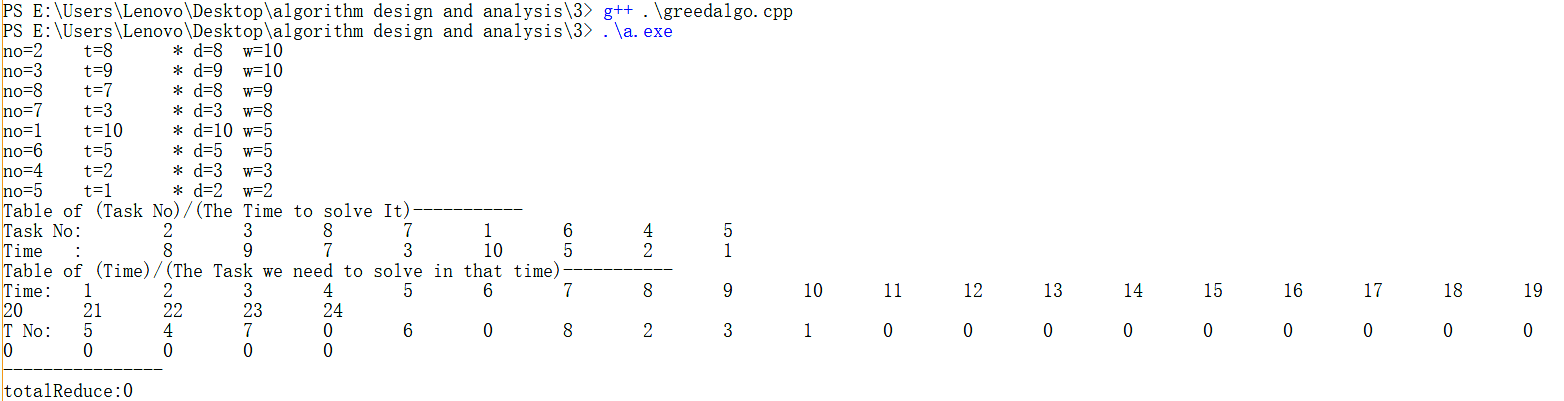
\includegraphics[scale=0.45]{greedalgo1.png}
\caption{单位时间作业安排问题的测试案例1}
\end{figure}
\begin{lstlisting}[language=C++,basicstyle=\footnotesize]
int d[N] = {
    2, 10, 15, 6, 7, 19, 14, 17, 12, 16, 
    24, 3, 18, 18, 3, 12, 9, 21, 21, 21,
    15, 16, 9, 2, 17, 18, 19, 20, 9, 20,
};
int w[N] = {
    21, 22, 14, 17, 20, 19, 20, 15, 21, 30,
    20, 23, 12, 11, 19, 13, 16, 10, 14, 13,
    12, 14, 11, 18, 18, 19, 15, 14, 13, 10,
};
\end{lstlisting}
\begin{figure}[H]
\centering
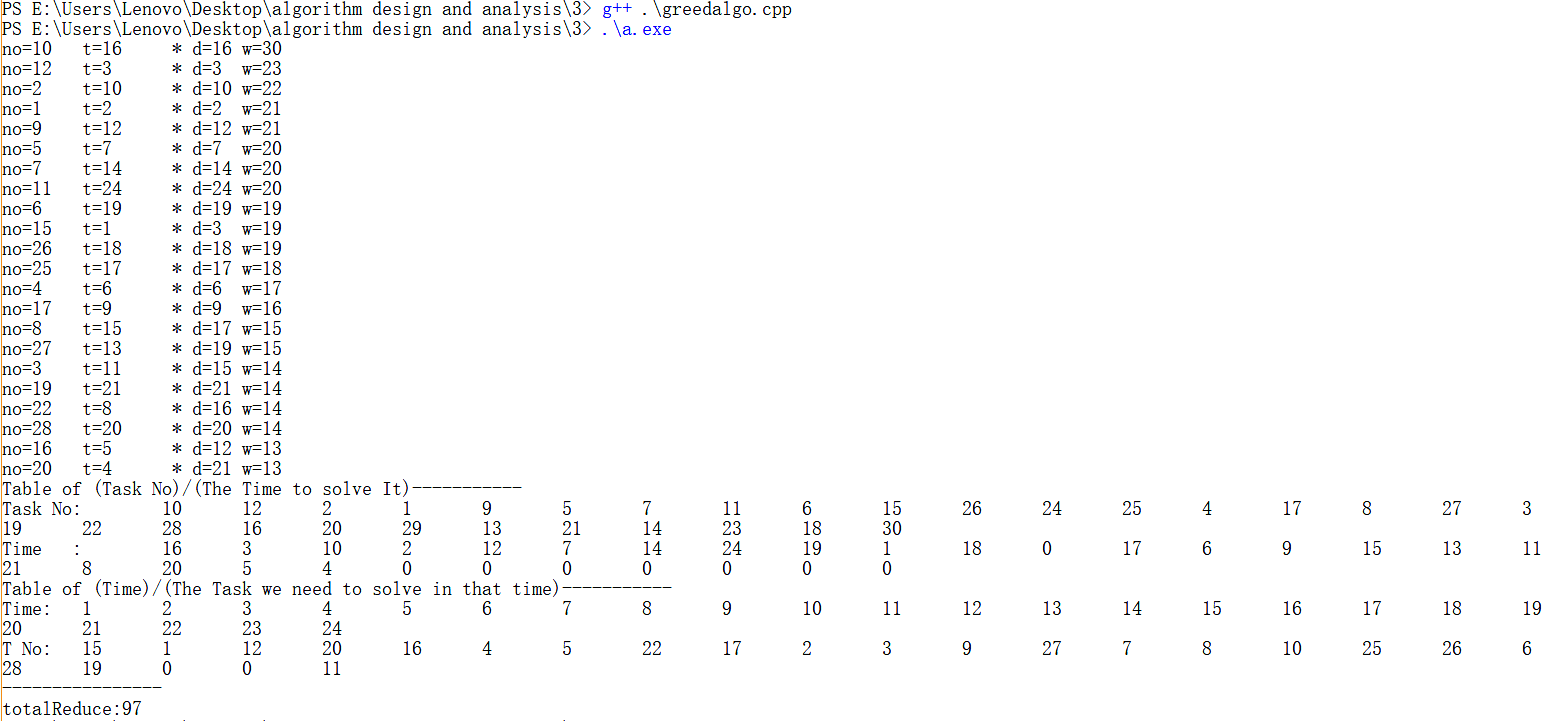
\includegraphics[scale=0.45]{greedalgo2.png}
\caption{单位时间作业安排问题的测试案例2}
\end{figure}

这两个案例前者是一个比较简单的例子,用于说明算法的正确性的,后者是更加符合题意的一个案例,具有足够多(30个)的作业需要考虑,这是明明肯定做不完的。所以他必须采用策略选择出一个可以使得总损失值最小的安排。

时间复杂度:$O(n^2)$,主要的时间都消耗在排序上了,这里我们采用的是冒泡排序,时间复杂度会较高一点,我们也可以采用具有归并排序或快速排序使得算法的时间复杂度下降为$O(nlog_n)$。

空间复杂度:$O(1)$,我们只采用了一个$finished[24]$来记录当前的选择情况,而$no[]$则是为了我们打印结果更加方便而额外准备的,所以只从结果上我们可以不考虑$O(n)$的$no[]$。

\section{讨论}

这个问题在求解过程中我们就可以感受到,这个问题也是可以采用动态规划的思想求解的,这里给出动态规划求解的递推表达式:

设$dp[i,d]$为当截止时间是$d$时,对于任务$\{1,2,\dots,i\}$具有的最小的总损失值。
$$
dp[i,d] = min\{dp(i-1,d)+w[i],dp(i-1,min\{d,d_i\}-t_i)\}
$$

当然,这里对于动态规划的解法,其最优子结构的证明和贪心算法的证明一样,而其重叠子问题可以通过递推表达式显而易见。这里也就不给出具体证明和算法的实现了。

\end{document}



